

\section{Introduction}
\label{sec:intro}


\begin{figure}[h]
    \vspace{-7pt}
    \centering
    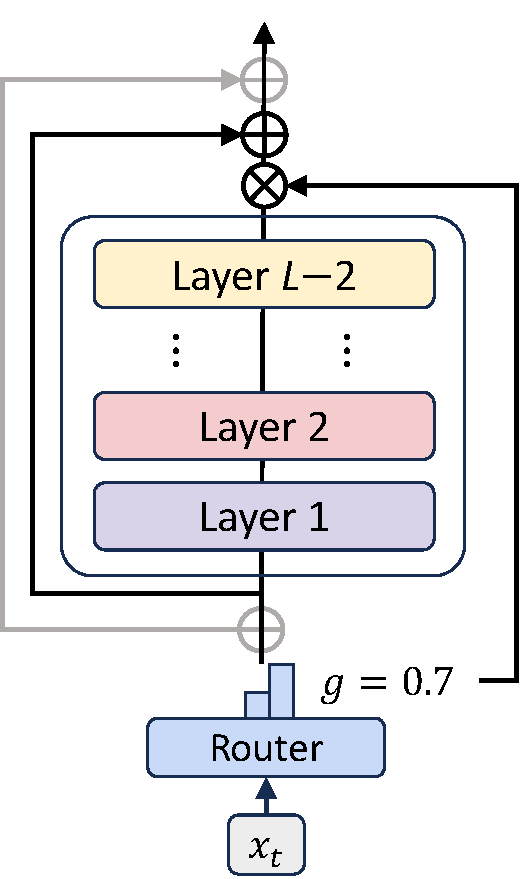
\includegraphics[width=0.23\columnwidth]{figs/overview/overview_main1.pdf}
    \hspace{23pt}
    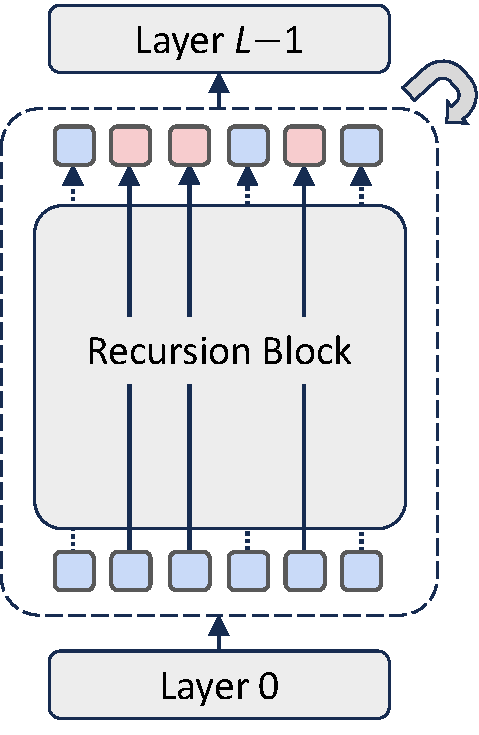
\includegraphics[width=0.238\columnwidth]{figs/overview/overview_main2.pdf}
    \hspace{7pt}
    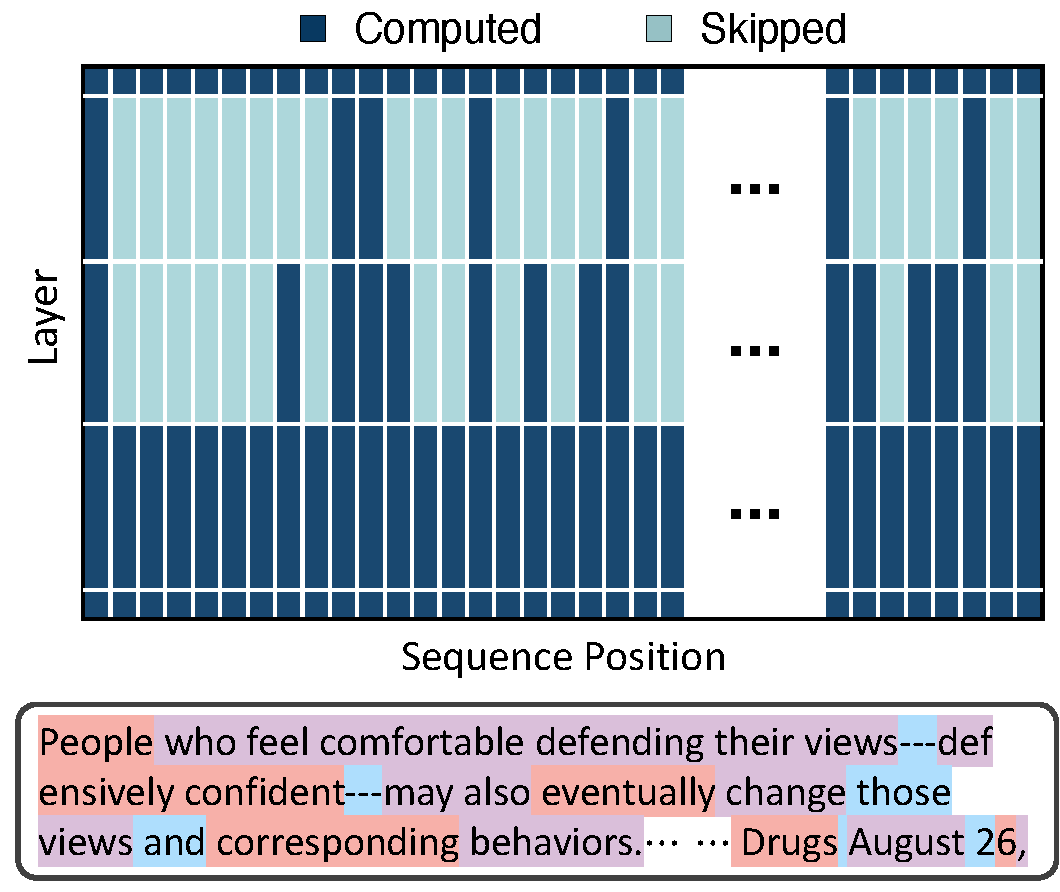
\includegraphics[width=0.43\columnwidth]{figs/overview/overview_main3.pdf}
    \caption{
    Overview of Mixture-of-Recursions (MoR). (\textit{Left}) Each recursion step consists of a fixed stack of layers and a router that determines whether each token should pass through or exit. This recursion block corresponds to the gray box in the middle.
    (\textit{Middle}) The full model structure, where the shared recursion step is applied up to $N_r$ times for each token depending on the router decision.
    (\textit{Right}) An example routing pattern showing token-wise recursion depth, where darker cells indicate active computation through the recursion block. Below shows the number of recursion steps that each subword token undergoes to predict the \textit{next} token, shown in colors: \raisebox{0pt}[0.5em][0.1em]{\colorbox{DarkOrchid!25}{1}}, \raisebox{0pt}[0.5em][0.1em]{\colorbox{SkyBlue!55}{2}}, and \raisebox{0pt}[0.5em][0.1em]{\colorbox{Salmon!60}{3}}. 
    }
    \label{fig:mor_overview}
\end{figure}



Scaling Transformer networks to hundreds of billions of parameters has unlocked impressive few-shot generalization and reasoning abilities~\citep{brown2020language, chowdhery2023palm, grattafiori2024llama, openai2023gpt4, reid2024gemini, deepseek-ai2024deepseek0v3, comanici2025gemini25pushingfrontier}.
However, the accompanying memory footprint and computational requirements make both training and deployment outside hyperscale data centers challenging~\citep{patterson2021carbon, momeni2024training}.
This has motivated researchers to seek alternative ``efficient'' designs~\citep{tay2022efficient, wan2023efficient}. 
Among the different axes of efficiency, \textit{parameter efficiency}~\citep{dehghani2018universal, bae2024relaxed, shazeer2017outrageously, fedus2022switch, lecun1989optimal}—reducing or sharing model weights—and \textit{adaptive computation}~\citep{raposo2024mixture, schuster2022confident, fedus2022switch, leviathan2023fast}—spending more compute only when it is needed—are promising, actively studied research directions.


One proven route to parameter efficiency is \textit{layer tying}, in which a shared set of weights is reused across multiple layers~\citep{dehghani2018universal, lan2019albert0, takase2021lessons, gholami2023generative, bae2024relaxed}.
For adaptive computation, a common approach is \textit{early-exiting}, which dynamically allocates compute by exiting  earlier in the network when predicting simpler tokens~\citep{elhoushi2024layerskip, schuster2022confident, Elbayad2020Depth-Adaptive, bae-etal-2023-fast}.
Despite the progress achieved along each of these individual efficiency axes, an architecture that effectively unifies both parameter efficiency and adaptive computation is still missing.
Recursive Transformers~\citep{bae2024relaxed, fan2024looped, giannou2023looped, yang2023looped, saunshi2025reasoning, geiping2025scaling, aleksandrov2025abbie}, models that repeatedly apply the same set of shared layers multiple times, offer a strong foundation due to their built-in weight sharing.
However, prior attempts at dynamic recursion have often been constrained by practical hurdles, such as requiring additional specialized training procedures or facing challenges in efficient deployment. This has led most approaches to still default to a simpler fixed-depth recursion, which applies the same amount of computation to every token and is thus incapable of delivering truly adaptive token-level compute allocation.


In this work, we introduce \textit{Mixture-of-Recursions} (MoR), a unified framework that fully leverages the potential of Recursive Transformers (see \autoref{fig:mor_overview}).
MoR trains lightweight routers end-to-end to assign token-specific recursion depths: it decides how many times a shared parameter block is applied to each token according to its required depth of ``thinking'', thereby directing computation to where it is most needed. 
This dynamic, token-level recursion inherently facilitates recursion-wise key–value (KV) caching, selectively storing and retrieving key–value pairs corresponding to each token’s assigned recursion depth. This targeted caching strategy reduces memory traffic, thereby improving throughput without relying on post-hoc modifications.
Therefore, MoR simultaneously (i) ties weights to cut parameters, (ii) routes tokens to cut redundant FLOPs, and (iii) caches key-values recursion-wise to cut memory traffic—all inside a single architecture.


Conceptually, MoR provides a \textit{pre-training} framework for latent space reasoning—performing non-verbal thinking by iteratively applying a single parameter block~\citep{hao2024training, geiping2025scaling, goyal2023think}. However, unlike approaches that deliberate on augmented continuous prompts before generation~\citep{liu2024deliberation, goyal2023think, hao2024training, shen2025codi}, MoR enables this latent thinking directly during the decoding of each token~\citep{zelikman2024quiet}. Furthermore, the routing mechanism facilitates adaptive reasoning along the model's vertical axis\footnote{While this thinking occurs along the depth axis, it is analogous to generating continuous thoughts along the horizontal sequence axis.}, moving beyond the uniform, fixed thinking depth common in prior work~\citep{geiping2025scaling, tack2025llm}. In essence, MoR enables models to efficiently adjust their thinking depth on a per-token basis, unifying parameter efficiency with adaptive computation.\looseness=-1


\vspace{-6pt}
\paragraph{Contributions.}
In summary, our key contributions in this paper are as follows.
\vspace{-3pt}
\begin{itemize}[leftmargin=*, itemsep=2pt]
    \item \textbf{Unified framework for efficient language modeling:} We present \emph{Mixture-of-Recursions} (MoR), the first architecture to unify efficiency paradigms—parameter sharing\,(\S\ref{subsec:preliminary}), token-level adaptive thinking depth\,(\S\ref{subsubsec:routing}), and memory-efficient KV caching\,(\S\ref{subsubsec:kv_cache})—within a single framework.

     \item \textbf{Dynamic recursion routing:} We introduce a router trained from scratch to assign dynamic per-token recursion depths. This aligns training with inference-time behavior and eliminates the need for costly, performance-degrading post-hoc routing stages used in conventional early-exit methods.

    \item \textbf{Extensive empirical validation:} Across models from 135M to 1.7B parameters\footnote{These are base model sizes, while MoR models have fewer unique parameters due to parameter sharing.} under equal compute budgets, MoR establishes a new Pareto frontier by improving validation loss and few-shot accuracy relative to vanilla and recursive baselines (\S\ref{subsec:main_results}, \S\ref{subsec:scaling_laws}).
    
    \item \textbf{Efficient architecture:} MoR dramatically reduces training FLOPs by selectively engaging only essential sequences in attention operations. Simultaneously, reduction in KV cache sizes leads to enhanced inference throughput itself, further boosted by continuous depth-wise batching (\S\ref{subsec:efficiency}).
    
\end{itemize}


